\subsection{Preprocessing}
Whenever data are recorded during an experiment, independently on the acquisition
system, it is necessary to perform some preprocessing tasks, in order to
remove the residual noise before performing the actual analysis on the data.\\
The steps commonly carried out during preprocessing are (not necessarily in this order):
\begin{itemize}
    \item Filtering
    \item Down-sampling
    \item Epoching
    \item Cleaning
    \item Artifacts rejection
    \item Referencing (mainly applied to EEG recordings)
\end{itemize}
\subsubsection{Filtering}
Filters are employed to select specific ranges of the signal or to remove unwanted frequencies,
such as the one at \(50\,Hz\), related to the electrical power supply. When filtering, it is
necessary to be careful, since it may bring some issues as well, as it affects the overall
data.\\
Several types of filters exist:
\begin{itemize}
    \item \textbf{High-pass filters:} remove the DC offset and slow trends in the data.
    \item \textbf{Low-pass filters:} remove high-frequency noise, performing an action
          similar to smoothing.
    \item \textbf{Notch (a.k.a. band-stop) filters:} remove the power line noise and its harmonics.
          It is a sort of extremely narrow band-pass filter.
    \item \textbf{Band-pass filters:} allow only a range of frequencies and remove the others.
          It is often obtained as a combination of high-pass and low-pass filters.
\end{itemize}
Some of the most important remarks about filters are:
\begin{itemize}
    \item IIR (infinite-impulse response) filters and FIR (finite-impulse response)
          filters are both valuable choices; however, FIR filters are commonly preferred
          whenever the phase distortion is an issue, as they do not introduce it, wheres
          IIR filters might. Therefore, FIR filters ensure a better phase-time relationship.
    \item In case of band-pass filters, it is critical to properly select the
          bandwidth of interest: in general broadband filters are preferred for neural
          signal in a high-frequency range, especially \(>30\,Hz\), as the activity
          is non-purely oscillatory, such as the multi-unit activity of neurons. When
          interested in low-frequency oscillations - i.e. alpha band or theta band - it is
          more effective to apply a narrowband filter (notch).
    \item Generally, notch filters have very low ranges of allowed frequencies and
          this might create artifacts and affect the signal in a negative way. Notice
          that by increasing the range of a band-stop filter, the power of the filter itself
          is reduced, leading to a worse removal of noise.
    \item Additionally, Morlet filtering is to be preferred when analysing the phase
          of multiple signals, as it employs narrowband filters, that allow a better reconstruction
          of the oscillation phase.
\end{itemize}
\subsubsection{Down-sampling}
After filtering, it might be useful to down-sample the data in order to reduce their size, decreasing
the computational load during the analysis. A critical issue to
take into account when down-sampling the signal is the Nyquist limit, such that
aliasing is avoided (i.e., the overlapping of subsequent harmonics).
\subsubsection{Epoching}
In many types of analysis it is common to divide the signal in equally long
non-overlapping chunks, which are denominated epochs. If these chunks are taken
by a common type of event, then they are denominated trials. Generally:
\begin{itemize}
    \item \textbf{Epochs:} partitions of the signal not related to a particular event.
    \item \textbf{Trials:} partitions of a signal defined around a specific event.
\end{itemize}
In both cases, the signal is divided into subsequent time windows with a fixed
length.
\begin{figure}[H]
    \centering
    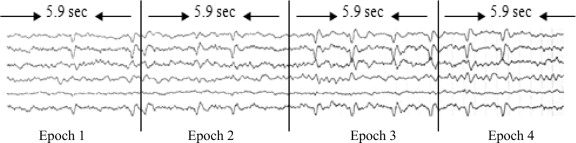
\includegraphics[scale=0.8]{12_1}
\end{figure}
A noticeable issue related to epoching is that taking a particular portion of
the signal corresponds to multiplying the overall signal for a rectangular window.
This introduces edges at the boundaries of the time window, which possibly results
in artifacts when filtering the epoch. This issue is particularly concerning when
the selected time window is short, due to the fact that the number of edges
(and consequently of artifacts) increases dramatically.
The optimal solution would consist in performing filtering before epoching. However,
in some types of analysis this might not be practical nor feasible, therefore two
distinct strategies exist to deal with the filtering of epochs:
\begin{itemize}
    \item Epochs might be created wider than the signal of interest, so that
          artifacts might be generated at the extremities of the epoched signal, but the
          centered portion of the signal, which is the one of interest, would not be affected.
          \begin{figure}[H]
              \centering
              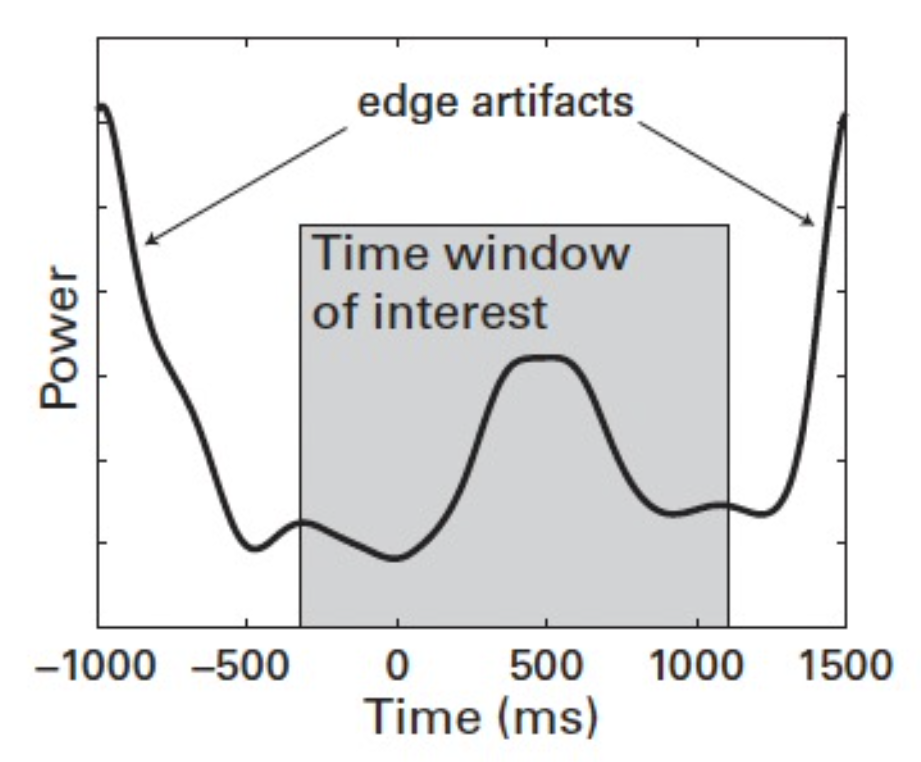
\includegraphics[scale=0.3]{12_2}
          \end{figure}
    \item Alternatively, the epoched signal might be replicated symmetrically both
          before and after itself (reflected signal). Then, the analysis might be performed
          without generating artifacts on the initial epoched signal (operating in a larger time
          window). Finally, the reflected portions of the initial signal can be discarded.
          \begin{figure}[H]
              \centering
              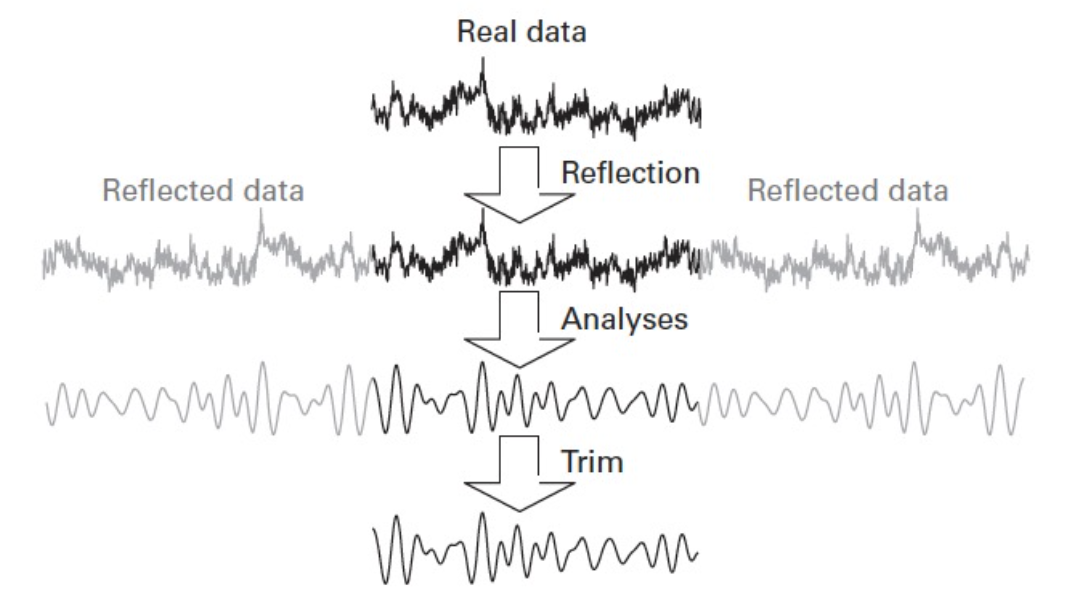
\includegraphics[scale=0.45]{12_3}
          \end{figure}
\end{itemize}
\subsubsection{Cleaning}
EEG and in general LFP recording techniques are much more prone to noise than
invasive technologies. In particular, other physiological activities might concur
in the noise, as they involve electrical activity as well, hence often they cannot be removed or isolated.
\begin{figure}[H]
    \centering
    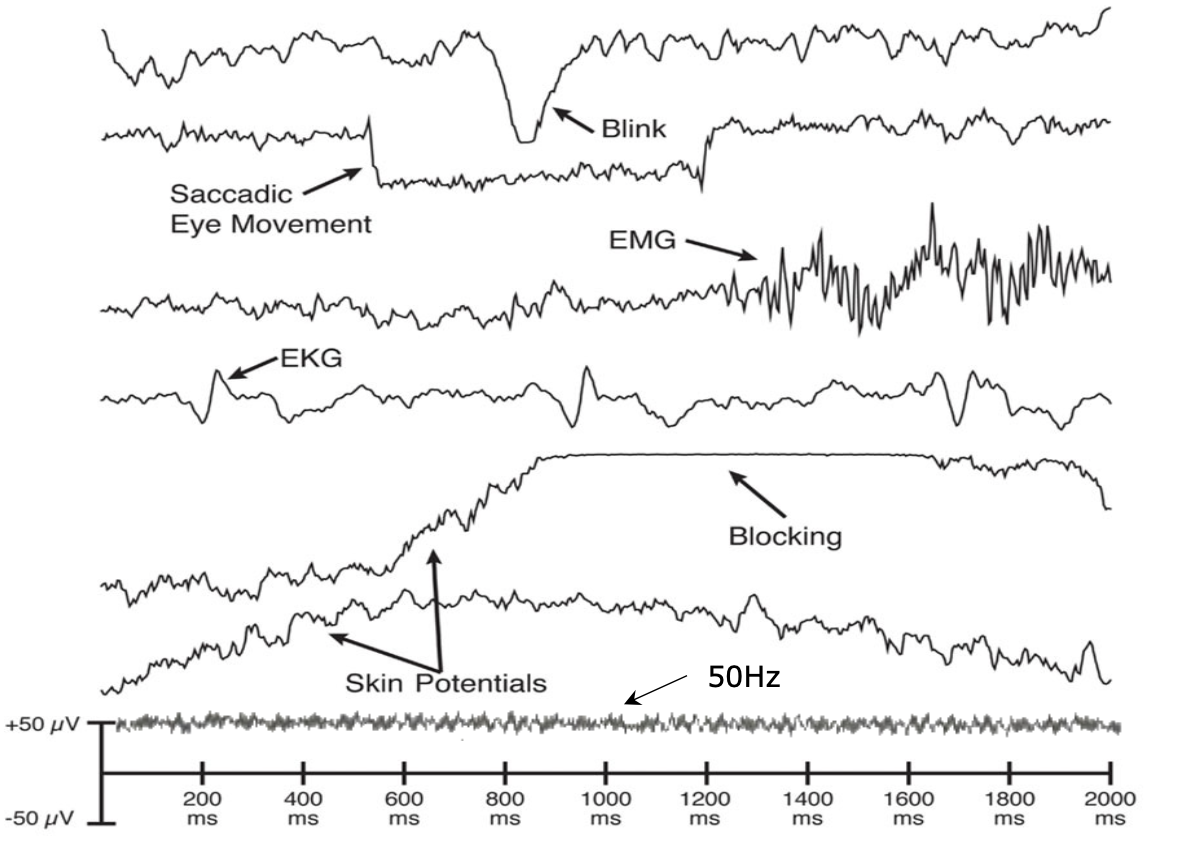
\includegraphics[scale=0.5]{12_4}
\end{figure}
\begin{itemize}
    \item \textbf{Blinking:} opening and closing the eyes generates clearly visible dipoles
          in the signal. This issue is especially observable in the channels referred to
          electrodes placed in the frontal part of the head, close to the eyes.
    \item \textbf{Saccadic eye movements:} rectangular-shaped artifacts are often found as a
          result of large saccades. Small saccades are generally not visible in EEG
          recordings. These artifacts are pretty easy to be identifies, due to their
          peculiar spatial distribution and duration.
    \item \textbf{EMG:} muscular activity is driven by electrical signals and they are often
          recorded by the EEG, especially when the muscles involved are the facial ones.
          An issue related to the EMG signals is that their frequency content is very similar
          to the one of the neural system, therefore they cannot be removed by a
          frequency-selective filtering.
    \item \textbf{EKG:} the electrical activity of the beating heart is larger in magnitude
          if compared to neural signals. These artifacts are characterized by a
          triangular shape and a specific orientation, related to the fact that the current flows
          in a particular direction (from posterior to anterior regions). They can be easily identified.
          Notice that also the flow of blood in the brain arteries is a source of noise.
    \item \textbf{Skin potential:} the impedance of the skin cannot be controlled.
    \item \textbf{Blocking:} the signal amplifier saturates, therefore it is not possible
          to properly record the signal, which instead becomes flat.
\end{itemize}
\subsubsection{Artifacts Rejection}
When dealing with artifacts, it is not always easy to identify them correctly, especially in
an automatized way. As a matter of fact, nowadays visual detection is usually still preferred.
Though visual identification of artifacts works well, it is extremely time consuming and
requires well-trained researchers. On the other hand, Independent Component Analysis (ICA) has
been suggested as a valid tool in identifying artifacts, as it enables to find the
independent sources of a signal. In the EEG case, ICA works as a spatial filter, trying to
separate the signal sources from a spatial point of view. Notice that the source separation
is performed by looking at the (variance) of the signal collected by all of the electrodes.
The signal from a generic electrode \(n\) in a set of \(N\) electrodes can be seen as the
sum of \(N\) independent components, each with a different weight - i.e. contributing in a
different manner to the overall recorded signal -:
\begin{equation*}
    n\text{-th electrode} = \sum_{i=1}^N w_{ni}\cdot{IC_i}
\end{equation*}
Therefore, each component is described by a weighted sum of the signal recorded by all the
electrodes. Then, it is possible to find those components isolating artifacts by visual
inspection (this works particularly well if the number of artifacts is quite low) and these
components are subtracted from the actual signals. In general, common artifacts such as blinks
and saccades are found in the first components, as their variance is particularly high if
compared to neural activity. Notice that the usual way to identify independent components
containing artifacts through visual inspection takes into account the topography of the signal,
its time course, and the frequency spectra.
\begin{figure}[H]
    \centering
    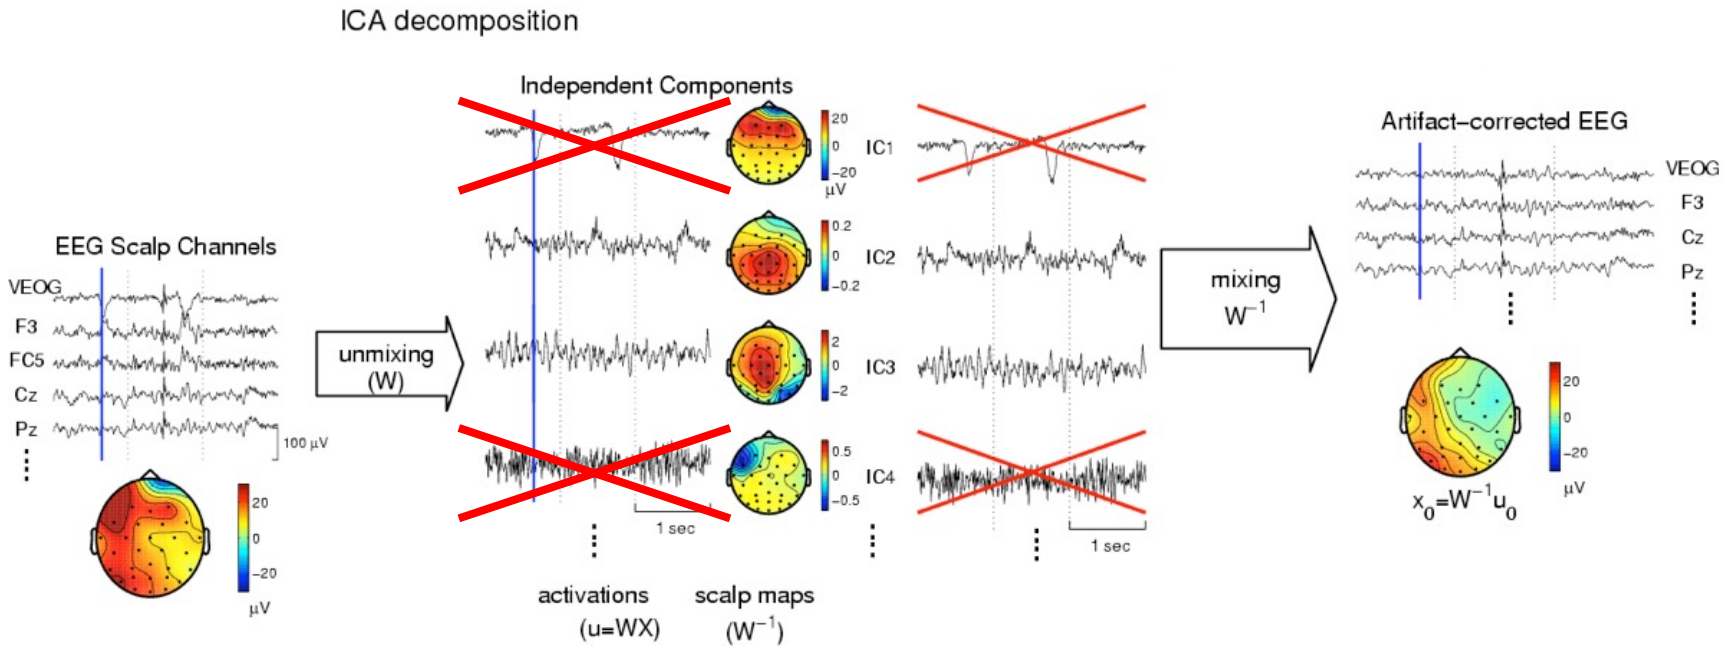
\includegraphics[scale=0.45]{12_5}
\end{figure}
\paragraph{ICA phase distortion} The Independent Component Analysis is a linear operator, thus
it is supposed not to distort or edit the phase of the signal. However, there is evidence
suggesting that ICA may adulterate the phase of data in EEG recordings which are supposed to
be clean. In particular, this represents an issue if:
\begin{itemize}
    \item \textbf{The number of recording channels is low:} if the number of channels is particularly
          low, the ICA algorithm might have difficulties in separating the
          sources in an effective way, failing in the research for artifacts.
    \item \textbf{The recording duration is short:} as above, a short recording implies a few number
          of samples, thus not enough data to allow an effective usage of ICA.
    \item \textbf{Inappropriate selection of artifactual components:} the components believed to
          contain artifacts are misjudged.
\end{itemize}
Let's point out once more that spatial filters - i.e. ICA - can change the phase relationship
between two channels. This is not an issue in absolute terms, however it is critical to
properly select the components to attenuate, such as the ones containing artifacts. The goal
is to enhance the SNR of the features of interest, while attenuating noise and artifacts.
\subsubsection{Referencing}
EEG signals are voltage differences between a specific point on the subject head and another
reference point. It is critical to select a proper positioning of the electrodes to have a
meaningful recording. The reference might be virtually any, nonetheless it is selected a
location displaying an activity similar to the once recorded by scalp electrodes.
The most common locations for the reference electrode are:
\begin{itemize}
    \item Earlobes
    \item Mastoids
    \item Nose
    \item Forehead
\end{itemize}
Another important electrode is the ground one, which can be placed anywhere on the head of the
subject.
\begin{figure}[H]
    \centering
    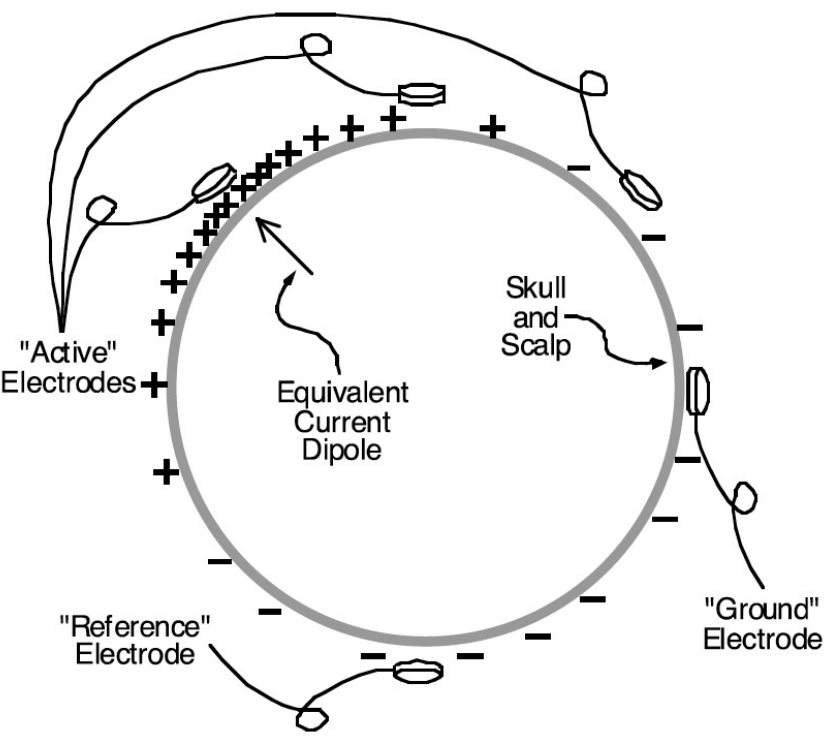
\includegraphics[scale=0.45]{12_6}
\end{figure}
The amplifiers employed in EEG recordings usually work through common-mode rejection
- i.e. an amplifier ability to individuate the noise common to different signals and remove
it -, which unluckily decades as the impedance increases. Therefore, it is fundamental to
have a low impedance between the recording electrodes and the subject skin: this is achieved
by enhancing their coupling via a conductive gel. Another vital aspects consists in having a
symmetric disposition of the electrodes on the head.\\
Notice that referencing is a linear operation, thus selecting a good referencing scheme is
crucial. There is no perfect scheme, it depends on the activity of interest which should be
recorded. Two distinct referencing approaches exist:
\begin{itemize}
    \item \textbf{Average scheme:} every channel is referenced to the average of the signals coming from
          all of the electrodes. This technique allows to remove the common activity recorded at
          each electrode: the common noise removal is strongly affected by the symmetry of the scheme.
          The major issue related to this method is that all the common activity is attenuated, not
          just noise: basically a smoothing filter is applied to the overall signal.
    \item \textbf{Laplacial spatial filter:} this electrodes scheme is preferred when a high-density
          EEG recording is performed. The reference for a generic electrode is taken as a weighted
          sum of the activity recorded by the nearby electrodes. This allows to obtain a
          well-localized activity. Notice that different shapes of the kernel - i.e. different
          neighbourhoods of electrodes - can be selected.
\end{itemize}

\subsection{Event-Related Potentials}
Once the pre-preprocessing is concluded, it is time to perform an actual analysis on the
recorded data. Three main types of analysis exist with respect to LFP signals:
\begin{itemize}
    \item \textbf{Activation:} study the activation of the brain, such as in response to a stimulus.
    \item \textbf{Conncectivity:} obtain hints about the interconnections between different
          areas of the brain.
    \item \textbf{Communication:} understand how different regons of the brain communicate
          with one another.
\end{itemize}
In this section, the main focus is activation, in particular a simple technique to investigate
it, known as Event-Related Potentials (ERPs).\\
ERP is a widely-spread way to analyse EEG evoked responses, which are the responses of the brain
when given a stimulus. It is a sort of black-box approach, as only the relationship between
input - i.e. the stimulus - and the output - i.e. the evoked potentials - is of interest.
ERPs is based on the hypothesis that the brain activity is event-related, thus the activity
observed after the stimulation is casused by the stimulus itself. As a consequence, everything
not cause by the stimulation is not replicated across time and can be considered noise.\\
Several trial of the same stimulation are recorded, each one ccontaining a temporal mixture
of signal and noise: signal is assumed to be consistent across trials referred to the same
stimulus. Thus, noise can be removed by averaging all the trials together. This can be done
as noise is assumed to be uncorrelated - i.e. it has no statistical meaning, thus it is random -
and centered around zero.\\
In this way, the Event-Related Potential is obtained: it exhibits both positive and negative
peaks, while oscillating around zero. Then, a correlation between peaks features, such
as temporal displacement and amplitudes, and events - i.e. stimuli - is investigated.
\begin{figure}[H]
    \centering
    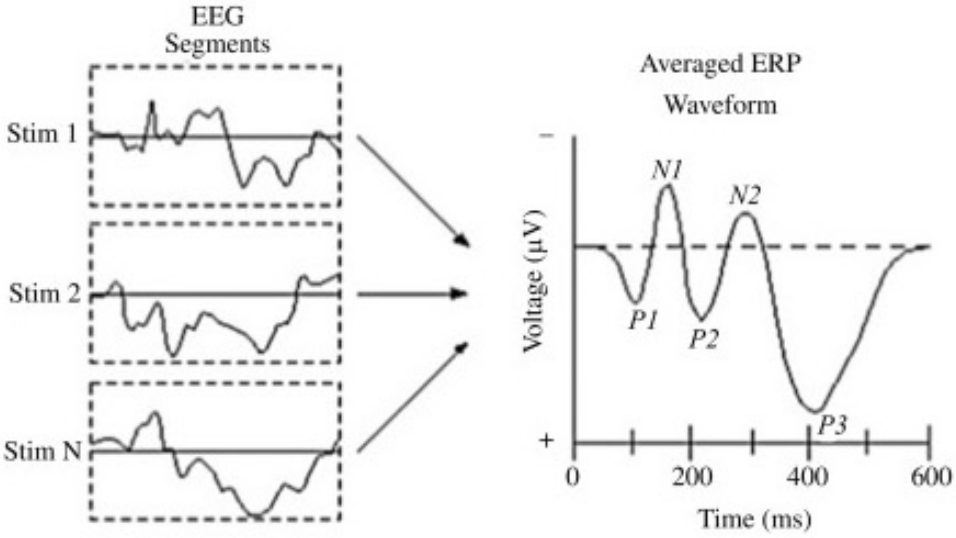
\includegraphics[scale=0.45]{12_7}
\end{figure}
Despite their effectivness, ERPs present some limitations and drawbacks. First of all, an
ERP does not provide any information concerning the frequency content of the response,
moreover the high-frequency components of the response are removed by the smoothing effect
given by the averaging of the trials, which works as a low-pass filter. A join time-frequency
representation can be obtained by exploiting either the Windowed Fourier Transform or the
Wavelet Trasform: in general the transofrm is applied to each trial and then the spectra
are averaged, by obtaining the so-called Event-Related Spectrum (ERS). It is then possible
to remove the baseline activity of the brain from the joint time-frequency representation,
producing a time-frequency representation exclusively for response to a perturbation
- i.e. the stimulus -, denominated Event-Related Spectral Perturbation (ERSP), which is
better described in the following pages.
Notice that a time-frequency representation is less significant for spontaneous activity,
while it is considerably informative in the presence of stimuli.
\begin{figure}[H]
    \centering
    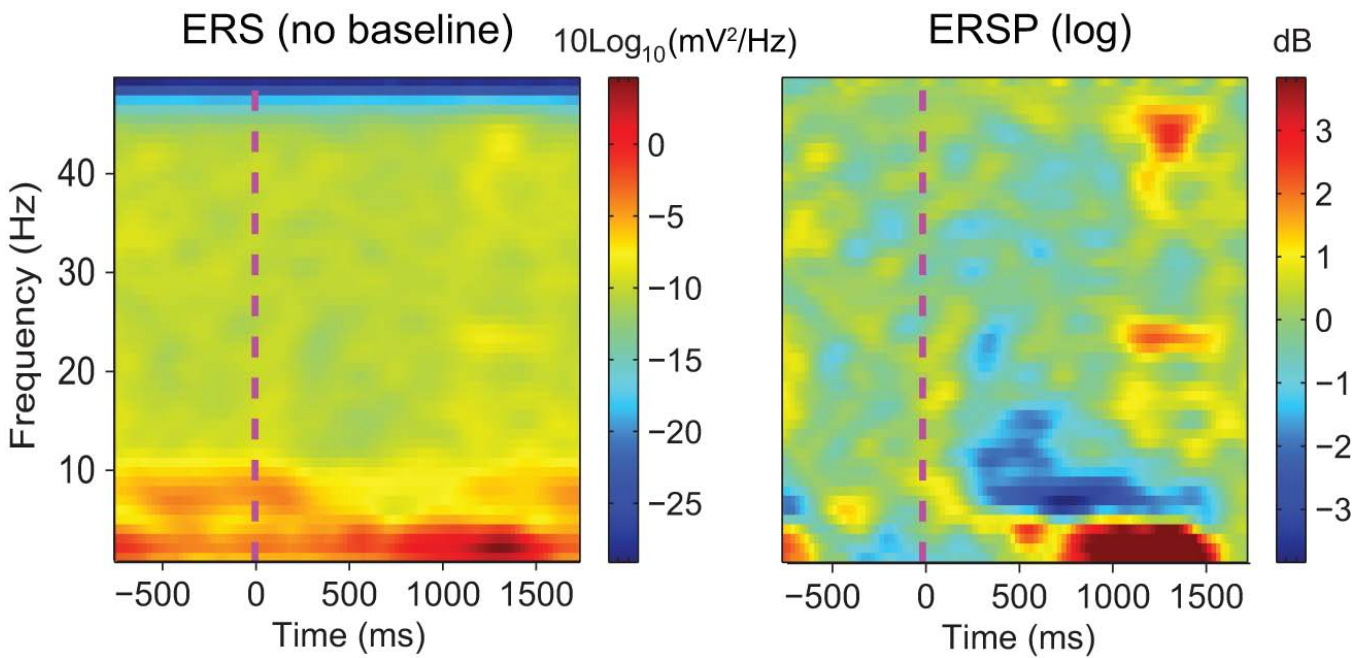
\includegraphics[scale=0.4]{12_8}
\end{figure}
\subsubsection{Global Field Power}
The evoked activity allows to look at the brain response after a single event, it is
common to consider every channel separately, by exploiting butterfly plots: the ERP for
each channel is plotted onto the same axes, allowing to quickly find the channels with
artifacts, as they will be significantly different from the average response.\\
Another choice to spot artifacts consists in taking into account the topographical variance
or Global Field Power (GFP) of the signal, which is the spatial variance on the activated
recording sites during an ERP by looking at the active channels.
\begin{itemize}
    \item \textbf{ERP:} the average of all channels across trials, resulting in a matrix that
          represents the number of channels and time.
    \item \textbf{GFP:} the variance across channels of the ERP matrix.
\end{itemize}
\begin{figure}[H]
    \centering
    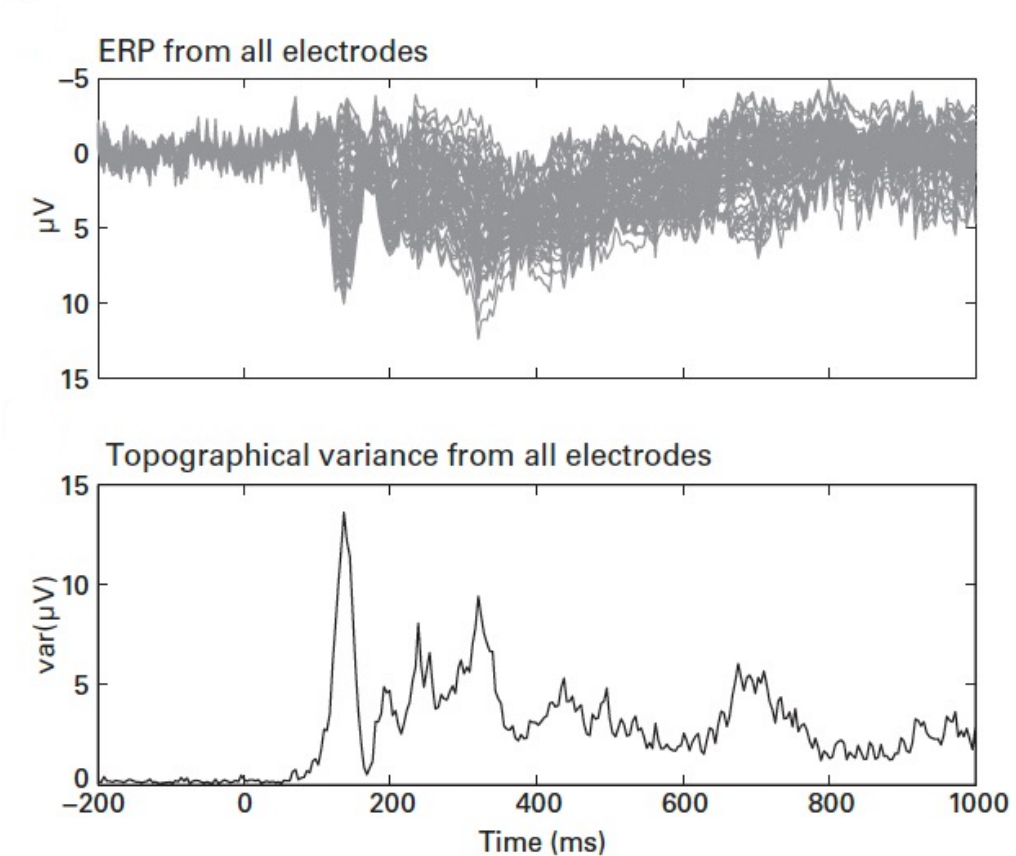
\includegraphics[scale=0.35]{12_9}
\end{figure}
\subsubsection{Baseline Normalization}
In the first place, let's define what baseline is: it represents the basal or spontaneous
activity recorded by a channel before the occurring of a stimulus. In many cases it might
be useful to compare the activity before - i.e. the baseline activity - and after - i.e. the
evoked response - a stimulus to understand how the neural system is affected by it.\\
In order to remove the baseline component from the evoked response, it has been suggested to
perform the so called basline normalization, consisting in removing the baseline contribution
from the after-stimulus signal. A normalized Event-Related Spectrum Perturbation can be
obtain as
\begin{equation*}
    ERSP_z(f,t)=\biggl(\frac{ERS(f,t)-\mu_B(f)}{\sigma_B(f)}\biggr)
\end{equation*}
where \(ERS(f,t)\) is the Event-Related Spectrum.
Other types of ERSP can be derived, such as the percentage difference between the basline
activity and the evoked response (a.k.a absolute ERSP)
\begin{equation*}
    ERSP_{\%}(f,t)=\frac{ERS(f,t)}{\mu_{B}(f)}
\end{equation*}
and the log-transformed ERSP measure
\begin{equation*}
    ERSP_{log}(f,t)=10\log_{10}\bigl(ERSP_{\%}(f,t)\bigr)
\end{equation*}
As shown below, the three ways to obtain a ERSP produce similar results, even if they
present some differences in the features they tend to enhance:
\begin{figure}[H]
    \centering
    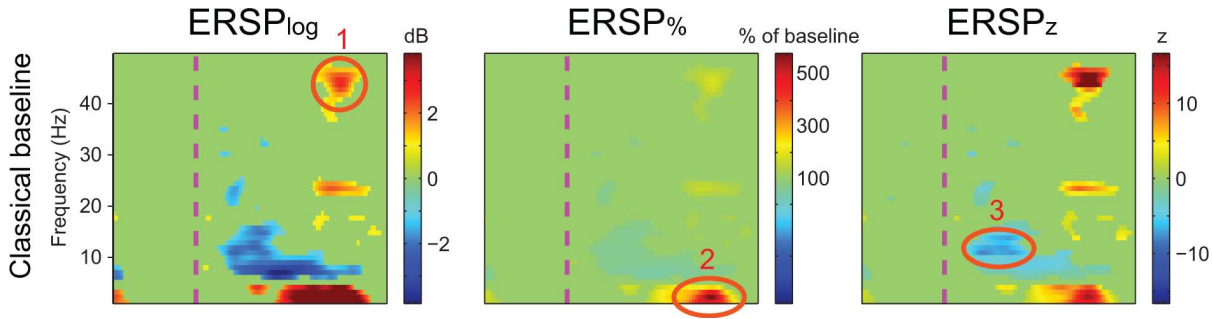
\includegraphics[scale=0.6]{12_10}
\end{figure}
\subsubsection{Filtering ERPs}
The topic of ERPs filtering is still a very debated one, as a number of issues might emerge:
\begin{itemize}
    \item \textbf{Distortion of response waveforms and emergence of spurious features:} if spurious
          features, such as delayed excursions or ringing, should emerge, they whould misleadingly
          suggest brain activity that is not really there.
    \item \textbf{Blurring of temporal relations (violation of causality):} the response latency is
          crucial to infer the sequence of neural events or the anatomical stage at which they
          occur. Rember that filters always introduce a delay.
    \item \textbf{Non-uniqueness of phenomenological descriptions:} they same event might be
          described in inconsistent ways according to the nature of the performed analysis and
          this would be a noticeable obstacle in comparisons between different studies. Moreover,
          the same phenomenon can be reported several times in a redundant way, as it would be
          disguised.
    \item \textbf{Lack of details to infer the processing involved:} methodological details
          on filtering would be necessary for a knowledgeable reader in order to fully understand
          the processing which took place.
\end{itemize}
Finally, remember that high-frequency filters might be problematic to employ when the goal is
to precisely track the dynamics of a signal.
\begin{figure}[H]
    \centering
    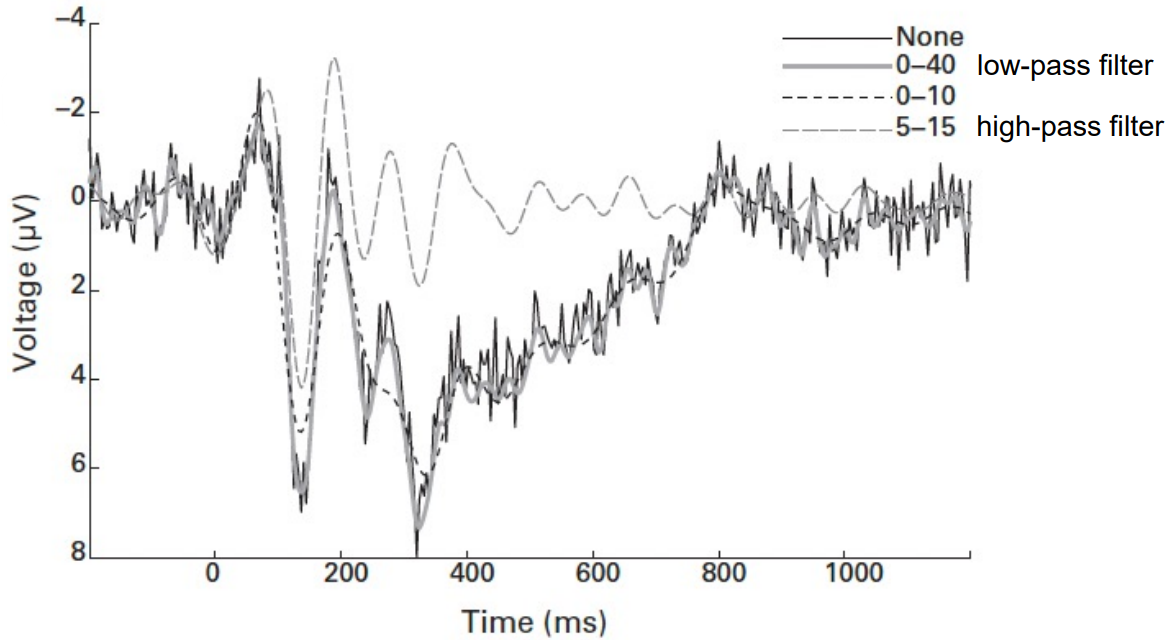
\includegraphics[scale=0.5]{12_11}
\end{figure}